\subsection{Wall Potentials} 

The simulation takes the natural behaviour of
avoiding to walk close to walls into account by using repulsive wall
potentials inversely proportional to the distance from the walls. 
Actually the walls are formed by a row of fixed agents. 
\[V_{wall}(r) = k_W  \frac{1}{r}\]
The range of the wall effect is restricted up to the distance $D_{max}$ from
the walls. This prevents taking a wall into account which is on the other side
of the room. $k_W$ is a constant, which describes, how strong the repulsive 
force of the wall is.

\subsection{Door Potentials}
The door potentials behave almost like the wall potential, the big difference
here is, that they are attracting. This means that they are proportional to
the square of the distance an agent is away from it.
\[V_{door}(r) = k_D (r + s)^2\]
$k_D$ is another constant describing the strength of the attracting force
caused by the door. The shifting $s$ factor is needed because the potential
mentioned above would have a zero gradient if the radius is zero. The door is
formed by a row of door agents which are uniformly distributed on the door's
width.

\subsection{People Potentials}
The potentials of the people is pretty much like the potential of the walls.
It also repels people, which are close.
\[V_{agent}(r) = k_A  \frac{1}{r}\]
What we used in our simulation is that the agents have an other constant $k_A$
in front of the $\frac{1}{r}$.

\subsection{Potential field}
All the various potentials result in a single force which acts on the agent.
The agent reacts according to this field and moves, as mentiond
above, along the negative gradient of the sum of all potentials.
The following pictures show how the static part of a room may look
like. The figure \ref{emptyRoom} illustrates an empty room. The static field of
this figure looks like the plots shown in figure \ref{contour} and \ref{3D}.
For these plots, the field was calculated, as if an agent was
heading for the door which is on the west side of the room \footnote{The plots
are limited to a maximum value of 2500. Otherwise the values could go up to 
infinity, if we hit a wall element exactly. In that case, we would not see
anything of the rest, just a plain area.}.
\begin{figure}
	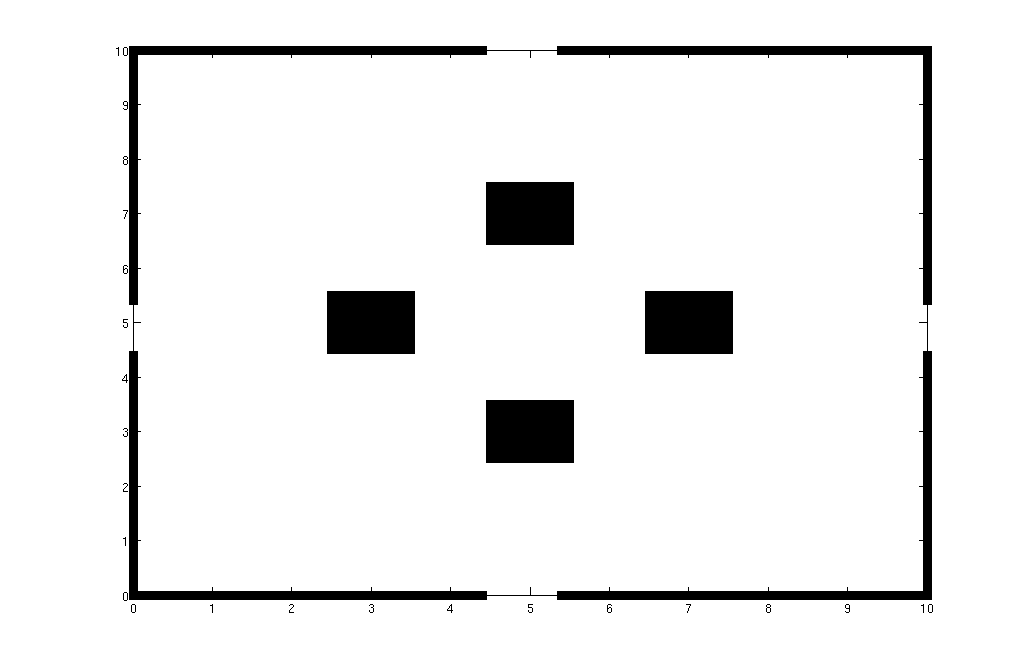
\includegraphics[width=\textwidth]{../graphen/emptyRoom.png}
	\caption{An example of an empty room}
	\label{emptyRoom}
\end{figure}
\begin{figure}
	\centering
	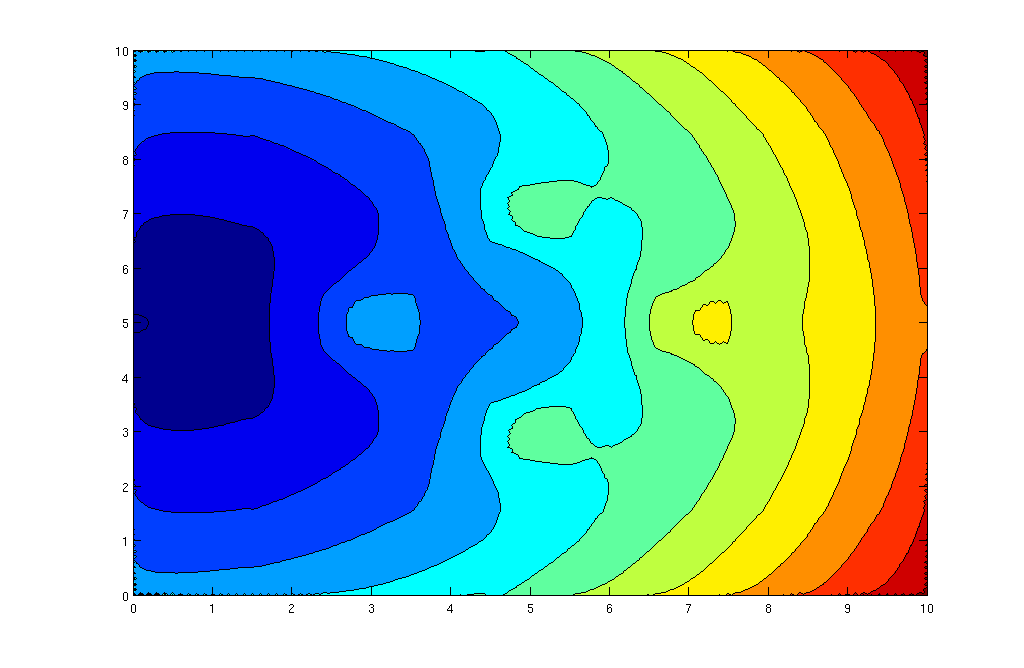
\includegraphics[width=0.8\textwidth]{../graphen/contour.png}
	\caption{Contour plot of room in figure \ref{emptyRoom}}
	\label{contour}
\end{figure}
\begin{figure}
	\centering
	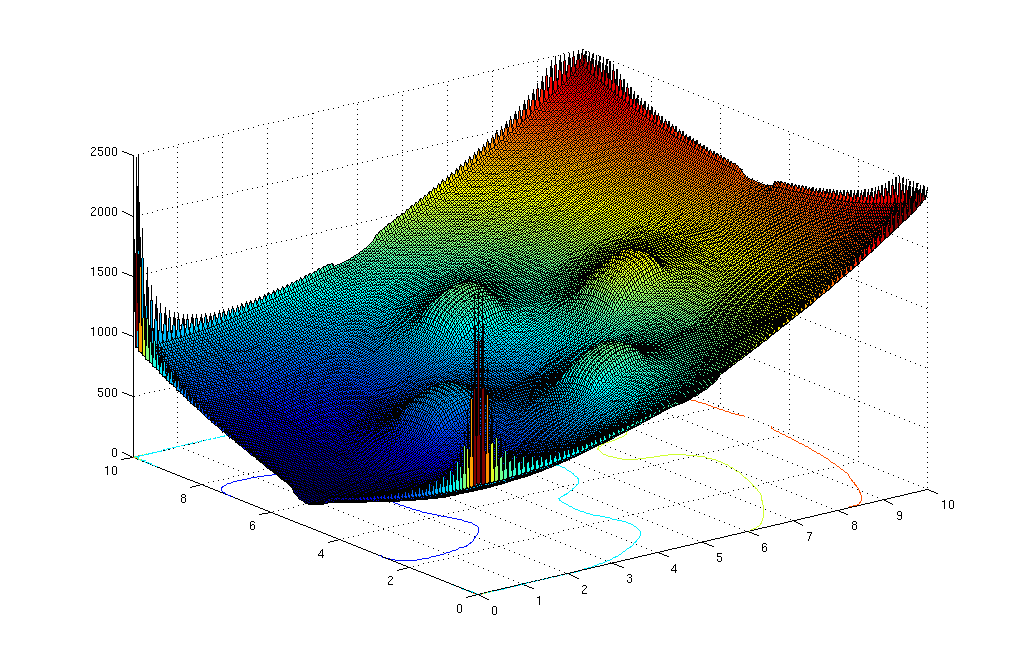
\includegraphics[width=0.8\textwidth]{../graphen/3DPotential.png}
	\caption{3D of static potential field of the room in figure
	\ref{emptyRoom}}
	\label{3D}
\end{figure}

If we also want to take the dynamic potentials into account, the room looks
like in figure \ref{10agentsContour} and \ref{10agents3D}. On those plots, the
room has been filled with ten agents at random positions.
\begin{figure}
	\centering
	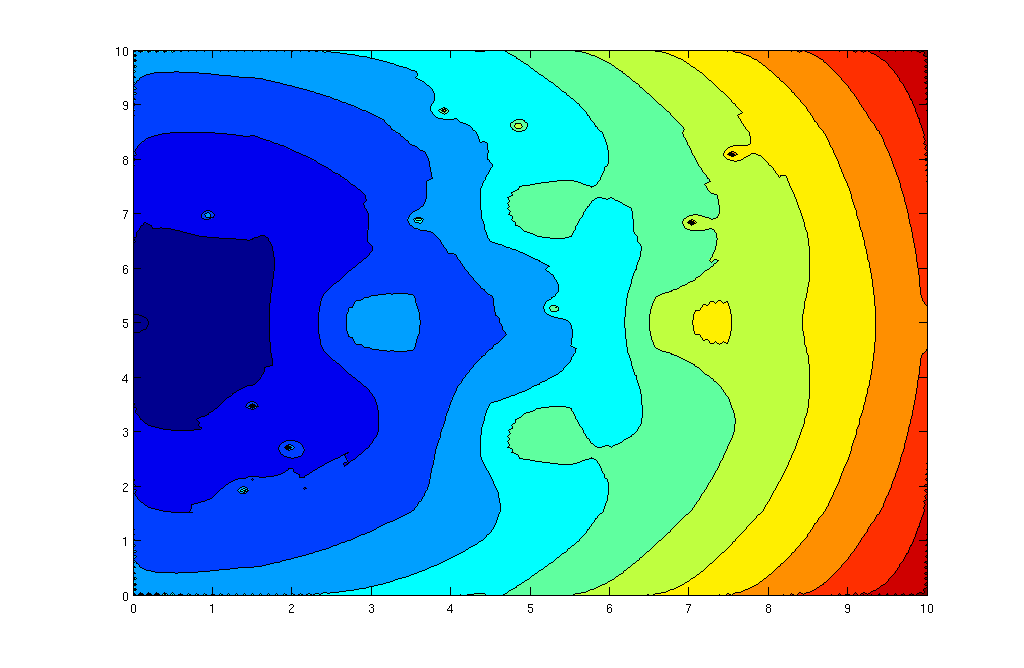
\includegraphics[width=0.8\textwidth]{../graphen/10agentsContour.png}
	\caption{Contour plot of room in figure \ref{emptyRoom} with 10 agents randomly positioned}
	\label{10agentsContour}
\end{figure}
\begin{figure}
	\centering
	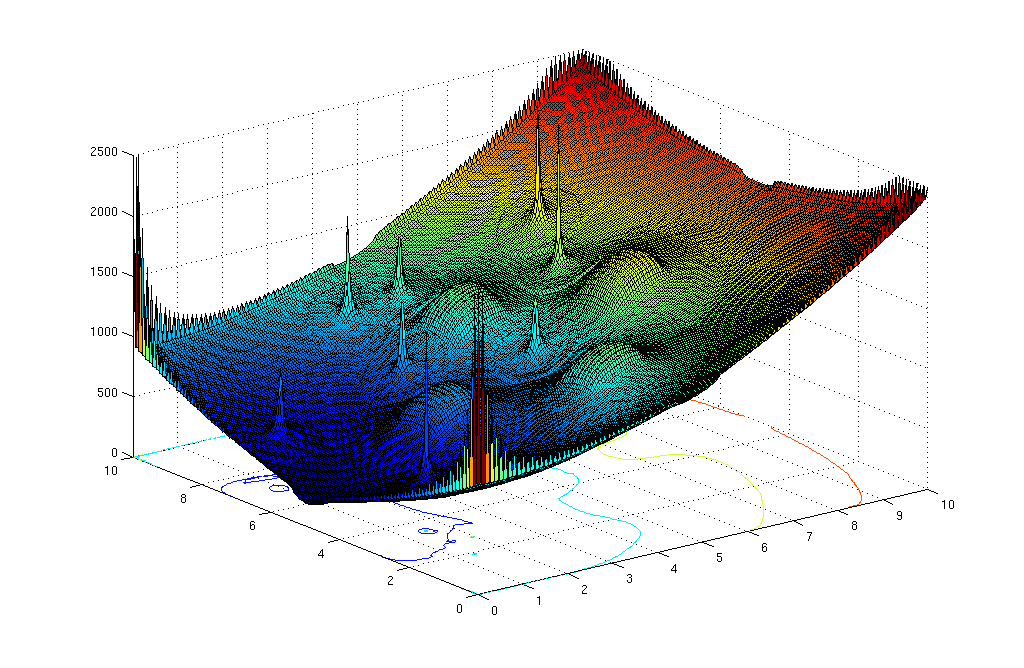
\includegraphics[width=0.8\textwidth]{../graphen/10agents3DPotential.png}
	\caption{3D of static potential field of the room in figure
	\ref{emptyRoom} with 10 agents randomly positioned}
	\label{10agents3D}
\end{figure}
